\documentclass[conference]{IEEEtran}
\usepackage{amsmath}
\usepackage{tikz}
\usetikzlibrary{arrows.meta,positioning,shapes.geometric}
\begin{document}
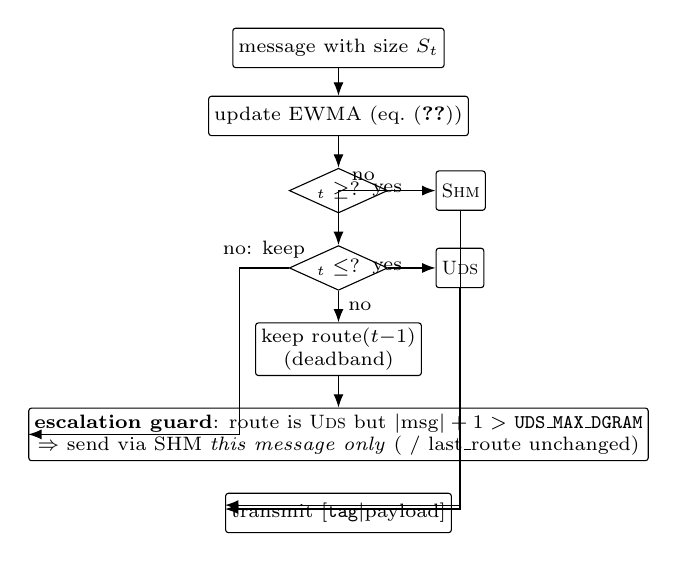
\begin{tikzpicture}[font=\scriptsize,>=Latex,node distance=4mm,
box/.style={draw,rounded corners=1pt,align=center,minimum height=5mm,
              inner sep=2pt},
  dec/.style={draw,diamond,aspect=2.2,align=center,inner sep=1pt}]
\node[box] (msg) {message with size $S_t$};
\node[box,below=3.5mm of msg] (upd) {update EWMA (eq.~\eqref{eq:ewma})};
\node[dec,below=4mm of upd] (d1) {$\sbar_t \geq \tauhigh$?};
\node[dec,below=4mm of d1] (d2) {$\sbar_t \leq \taulow$?};
\node[box,right=6mm of d1] (shm) {\textsc{Shm}};
\node[box,right=6mm of d2] (uds) {\textsc{Uds}};
\node[box,below=4mm of d2] (sticky) {keep $\mathrm{route}(t{-}1)$\\(deadband)};
\node[box,below=4mm of sticky] (eg) {\textbf{escalation guard}: route is
  \textsc{Uds} but $|{\rm msg}|+1 >$ \texttt{UDS\_MAX\_DGRAM}\\
  $\Rightarrow$ send via SHM \emph{this message only}
  ($\sbar$ / last\_route unchanged)};
\node[box,below=4mm of eg] (tx) {transmit [\texttt{tag}$\mid$payload]};
\draw[->] (msg) -- (upd);
\draw[->] (upd) -- (d1);
\draw[->] (d1) -- node[left]{yes} (shm);
\draw[->] (d1.east) -| node[above,pos=0.25]{no} (d2.north);
\draw[->] (d2) -- node[left]{yes} (uds);
\draw[->] (d2.south) -- node[right]{no} (sticky.north);
\draw[->] (d2.west) -| node[above,pos=0.25]{no: keep} ([xshift=-2mm]sticky.west)
          |- (eg.west);
\draw[->] (shm.south) |- ([yshift=1mm]tx.west);
\draw[->] (uds.south) |- ([yshift=0.5mm]tx.west);
\draw[->] (sticky) -- (eg);
\end{tikzpicture}
\end{document}
